\documentclass[12pt,a4paper]{article}
\usepackage[utf8]{inputenc}
\usepackage[ngerman]{babel}
\renewcommand\thesection{\arabic{section}}
\usepackage{graphicx}
\usepackage{amsmath}
\usepackage{amsfonts}
\usepackage{amssymb}
\usepackage{dsfont }
\usepackage{color}
\usepackage{hyperref}
\usepackage{subfigure}
\usepackage{wrapfig}
\usepackage[onehalfspacing]{setspace}
\usepackage{biblatex}
\addbibresource{myreferences.bib}
\setlength{\parindent}{0pt}

\title{Optimal Exercise Boundary für Amerikanische Optionen}
\author{Leander Piepenbring - Minh Anh Le }
\date{Wirtschaftsmathematik - HTW Berlin\\\\Februar 2022 }

\begin{document}
\setcounter{tocdepth}{1}
\newpage
\maketitle
\newpage
\tableofcontents
\newpage
\listoffigures   
\newpage
\part{\centering Einleitung}
\section{Optionen}
\begin{text}

Optionen sind Finanzderivate, die sich auf einen zugrunde liegenden\\ Vermögenswert beziehen, wie z.B eine Aktie $S$. Die Option besteht aus einem Vertrag zwischen zwei Parteien, einem Käufer und einem Verkäufer. Der Verkäufer gibt dem Käufer die Möglichkeit eine Aktie zu einem bestimmten Preis (Strikepreis $K$) zu kaufen, wenn es sich um eine Call-Option handelt. Handelt es sich bei der Option um eine Put-Option, hat der Käufer das Recht eine Aktie zu einem bestimmten Preis $K$ zu verkaufen. Wenn der Käufer dieses Recht in Anspruch nimmt, redet man von der Ausübung der Option. Der Preis für dieses Recht, ist der Optionspreis, oder auch Prämie genannt.
\\\\
Wenn man in eine Call-Option investiert spricht man von einer Long-Position. Der Käufer dieser Option profitiert davon, wenn der Preis der zugrunde liegenden Aktie steigt. Eine Investition in Put-Optionen nennt man Short-Position. In diesem Fall profitiert der Halter der Option davon, dass der Preis der Aktie fällt.
\\[0.3cm]
\begin{figure}[h]
\begin{center}
 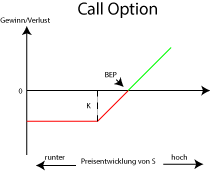
\includegraphics[width=0.4\textwidth]{CallOption.png}
 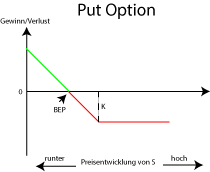
\includegraphics[width=0.4\textwidth]{PutOption.png}
 \caption{Call - und Put Option}
\end{center}
\end{figure}
\\\\
Da Optionen sich immer auf einen zugrunde liegenden Vermögenswert beziehen, hängt der Preis der Option stark von dem Preis dieses Vermögenswertes ab. Put-Optionen sind auch deswegen sehr beliebt, weil sie die Möglichkeit bieten, sich vergleichsweise einfach gegen starke Marktkorrekturen abzusichern.
\\\\

\section{Amerikanische Optionen}
Grundsätzlich gibt es verschiedene Optionen: Europäische-, Amerikanische- und Asiatische Optionen sind wohl die bekanntesten. Der Schwerpunkt dieses Projekts liegt aber auf den Amerikanischen Optionen. Amerikanische - und Europische Optionen ähneln sich von ihrem Profil her am stärksten. Der Unterschied zwischen den beiden liegt nur darin, wann die Optionen ausgeübt werden können. 
\\\\
Bei Europäischen Call - und Put Optionen, kann der Besitzer der Option sein Optionsrecht nur einmalig am Ende der Laufzeit $T$ ausüben. Dadurch, dass der Ausübungszeitpunkt festgelegt ist, hängt der Preis der Option nur von der Auszahlung im Zeitpunkt $T$ ab. Für die Berechnung der Preise von Europäischen Call - und Put Optionen wurde die Black-Schols Formel entwickelt.
\\
Amerikanische Optionen dagegen, können zu jedem beliebigen Zeitpunkt innerhalb der Laufzeit ausgeübt werden. 
\\\\

\newpage
\section{Problemstellung}
Aufgrund des variablen Ausübungszeitpunktes, ist die Bewertung von Amerikanischen Optionen wesentlich komplexer, als bei Europäischen Optionen. Da die Optionen zu jedem Zeitpunkt innerhalb der Laufzeit ausgeübt werden können, muss das Auszahlungsprofil $K-S$ (Put-Option), $S-K$ (Call-Option) herangezogen werden und mit dem Erwartungswert, der sich durch zukünftige mögliche Auszahlungen ergibt verglichen werden. Für diese Art von Problem ist es nicht möglich, eine analytische Lösung zu finden, weshalb numerische Methoden benötigt werden.
\\[0.3 cm]
Ein großer Anteil der Optionen die heutzutage gehandelt werden sind Amerikanische Optionen. Deshalb ist eine effiziente Methode zur Bestimmung der Optionspreise notwendig.
\\[0.3 cm]
In diesem Projekt soll die optimale Ausübungsumgebung für Amerikanische Optionen ermittelt werden. Die optimale Ausübungsumgebung oder auch Optimal Exercide Boundary genannt, ist die Grenze, die dem Investor aufzeigt, ob er seine Option ausüben oder weiter halten sollte. Ein Modell, in dem die Preisentwicklung von Amerikanischen Optionen sehr gut veranschaulicht wird, ist das Binomial Modell.
\\[0.3 cm]
Der Code für dieses Projekt wurde in Python implementiert.

\newpage
\part{\centering Methode}
\section{Einführung in das Binomialmodell}
Das Binomialmodell ist die am häufigsten verwendete Methode, um einen Arbitrage-freien Preis der amerikanischen Put-(Call) Option zu finden. In dem Projekt wird das n-Perioden Binomialmodell verwendet, das unter dem Name CRR-Modell bekannt ist. Es funktioniert durch die Konstruktion eines Baums, der verschiedene Aktienkurse vom Ausgangszeitpunkt $t_0$ = 0 bis zum Fälligkeitszeitpunkt T darstellt. Das Modell basiert auf dem Anfangkurs einer Aktie und geht dann davon aus, dass der Aktienkurs zu einem bestimmten Zeitpunkt steigen oder fallen wird, wodurch eine Baumstruktur entsteht.
\\\\ Der Preis der Aktie kann sich pro Periode um die konstanten Raten u und d verändern. Der Fall, dass der Aktienkurs steigt ist $u$ (up) und trifft mit einer Wahrscheinlichkeit von $p$ ein.
\\
Der Fall, in dem der Preis der Aktie fällt ist $d$ (down) und trifft mit der \\Wahrscheinlichkeit $1-p$ ein. $0 < p < 1$
\\\\
Sei $B_{t_i} = (1+r)^i$ der Preis eines risikolosen festverzinslichen Wertpapiers zum Zeitpunkt t, wobei $r \in R $ die konstante Zinsrate und $i = 0,1,...,n$ ist.
\\
Um \textbf{Arbitragefreiheit} zu gewährleisten muss immer $d < 1+r < u$ erfüllt sein. Weiter lässt sich das risikoneutrale Wahrscheinlichekeitsmaß $p$ durch $p = \frac{R-d}{u-d}$ berechnen, wobei $R = e^{r\cdot dt}$ dem Zinssatz pro Periode entspricht. Dieser Wert entspricht der Wahrscheinlichkeit einer Aufwärtsbewegung.
\\\\
Sei weiter $S(i,j) = (S_0 \cdot u^{i} \cdot d^{i-j})$ der Preis der zugrunde liegenden Aktie im Zeitpunkt i, wobei $0<j<i$ . Der Preis ergibt sich also durch Multiplikation des Preises der Aktie in $t=0$ mit der Anzahl der Aufwärtsbewegungen $u^{i}$ und der Anzahl der Abwärtsbewegungen $d^{i-j}$.

\begin{figure}[h]
\begin{center}
 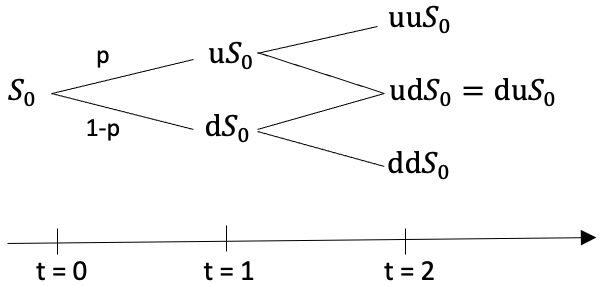
\includegraphics[width=0.8\textwidth]{BinomialModell.png}
 \caption{Beispiel Binomialmodell}
\end{center}
\end{figure}

\newpage

\section{Optionspreis im Binomialmodell}
Wenn man nun den Wert einer Amerikanischen Option in einem bestimmten Zeitpunkt bestimmen möchte, muss man sowohl den inneren Wert, als auch den Erwartungswert der Option berechnen.
\\\\
Um jeden Knoten im Baum zu identifizieren definieren wir $(i,j)$, wobei $0\leq i\leq n$ die Periode angibt, in der sich der Knoten befindet und $0\leq j\leq i$ die Anzahl der Aufwärtsbewegungen definiert. Sei im folgenden $C(i,j)$ der Preis einer Call Option und $P(i,j)$ der Preis einer Put-Option in einem bestimmten Knoten.
\\\\
Der innere Wert der Optionist die Differenz zum Strikepreis K, zu dem die Option ausgeübt werden kann. 
\begin{center}
    $X_C$(i,j) = $(S \cdot u^j \cdot d^{i-j} - K)^+$\\
    $X_P$(i,j) = $(K - S \cdot u^j \cdot d^{i-j})^+$
\end{center}
Das Pluszeichen zeigt, dass die Klammern immer gleich oder größer als Null sind. Das bedeutet, dass die Option keine negative Auszahlung hat. Der theoretische Gewinn einer Call-Option ist unbegrenzt, während er bei einer Put-Option durch den Strikepreis K begrenzt ist.
\\\\
Der Erwartungswert ergibt sich durch Rückwärtsrechnung durch den Baum.
Der Preis einer Call-Option $C(i,j)$ und einer Put-Option $P(i,j)$ zu einem Zeitpunkt $t$ ist nach dem Erwartungswert gegeben durch:
\begin{center}
$\mathbb{E}_C(i,j)} = \frac{1}{R} \cdot (p\cdot C(i+1,j+1) + (1-p)\cdot C(i+1,j))$
\\[0.3 cm] 
$\mathbb{E}_P(i,j)} = \frac{1}{R} \cdot (p\cdot P(i+1,j+1) + (1-p)\cdot P(i+1,j))$
\end{center}
Da amerikanische Optionen zu jedem Zeitpunkt innerhalb der Laufzeit ausgeübt werden können, entspricht der Wert der Option, dem Maximum von Erwartungswert - und innerem Wert. 
\\
Für eine amerikanische Call-Option $C(i,j)$ ergibt sich also:

\begin{center}
    \textbf{C(i,j)} = $max \{\hspace{0,2 cm} X_C(i,j) \hspace{0,2 cm};\hspace{0,2 cm}\mathbb{E}_C(i,j) \hspace{0,2 cm}\}$
    \\[0.3 cm] 
     = $max \{(S \cdot u^j \cdot d^{i-j} - K)^+ ; \frac{1}{R} \cdot (p\cdot C(i+1,j+1) + (1-p)\cdot C(i+1,j)) \}$ \end{center} 
\\
und für eine amerikanische Put-Option $P(i,j)$:

\begin{center}
    \textbf{P(i,j)} = $max \{\hspace{0,2 cm} X_P(i,j) \hspace{0,2 cm};\hspace{0,2 cm}\mathbb{E}_P(i,j) \hspace{0,2 cm}\}$
    \\[0.3 cm] 
    = $max \{(K - S \cdot u^j \cdot d^{i-j})^+; \frac{1}{R} \cdot (p\cdot P(i+1,j+1) + (1-p)\cdot P(i+1,j)) \}$  
\end{center}
\raggedlift
Diese Art, den Wert von amerikanischen Optionen zu bestimmen ist allerdings nicht effizient genug, weil die Optionen immer eine positive Wahrscheinlichkeit haben, früher ausgeübt worden zu sein.
\\
Aus diesem Grund soll nachfolgend eine effizientere Methode vorgestellt werden, um die Optimale Ausübungsumgebung zu bestimmen.

\newpage
\part{\centering Optimal Exercise Boundary in einem Binomial Modell}   
\section{Stopping-Region und Hold-Region}\footnote[1]{Kim and Byun 1994, S.140}\\
Im folgenden betrachten wir eine Amerikanische Put-Option.
Als ersten müssen zwei Regionen definiert werden, die Hold-Region $\mathcal{H}$, in der es vorteilhalft ist, die Option weiter zu halten und die Stopping - Region $\mathcal{S}$, in der die Option ausgeübt werden sollte.\\
\begin{itemize}
    \item \centering{$\mathcal{S}$} = $ \{ (i,j) \hspace{0,3 cm} \vert \hspace{0,3 cm} \textbf{P(i,j)} = (K - S \cdot u^j \cdot d^{i-j})^+ \}$
    \item \centering{$\mathcal{H}$} = $ \{ (i,j) \hspace{0,3 cm} \vert \hspace{0,3 cm} \textbf{P(i,j)} > (K - S \cdot u^j \cdot d^{i-j})^+ \}$
\end{itemize}

\begin{figure}[h]
\begin{center}
 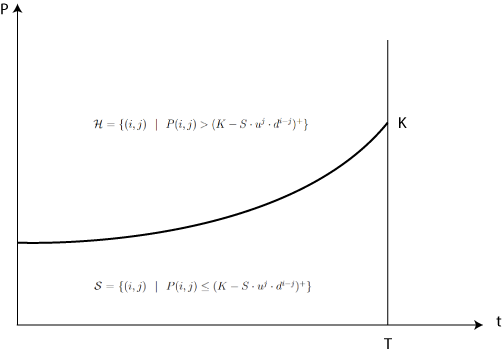
\includegraphics[width=0.7\textwidth]{BoundaryBild.png}
 \caption{Stopping-,Hold-Regionen}
\end{center}
\end{figure}
\\
\raggedlift Wenn der innere Wert der Option größer oder gleich dem Erwartungswert ist, soll die Option ausgeübt werden. Falls der Erwartungswert größer als der innere Wert ist, soll die Option weiter gehalten werden.



\section{Optimal exercise boundary}  
\underline{Was ist Optimal exercise boundary \footnote[2]{Basso 2001, S.7-8} ?}\\\\
Sei $\mathcal{I}$ die Menge der Zeitpunkte $i$, in denen es mindestens einen Stoppknoten gibt.
\begin{center}
         $\mathcal{I} = \{ \hspace{0,1 cm} i \hspace{0,2 cm} \vert \hspace{0,2 cm} \exists j :  (i,j) \in \mathcal{S} \hspace{0,1 cm}\} $ , wobei $0 \leqslant j \leqslant i. $
\end{center}
Daraus folgt, dass es für jedes $ i \in \mathcal{I} $ einen Zustand $B(i)$ gibt, sodass $(i,j) \in \mathcal{H}$ \hspace{0,2 cm} für  $j > B(i)$ und $(i,j) \in \mathcal{S}$ für  $j < B(i).$ Deshalb wird $B(i)$ definiert als:
\begin{center}
    $B(i) = max \{ \hspace{0,1 cm} j \hspace{0,2 cm} \vert \hspace{0,2 cm} (i,j) \in \mathcal{S} \hspace{0,1 cm}\} $ 
\end{center}
\\
der optimale Ausübungszustand (optimal exercise state) für jedes $ i \in \mathcal{I} $. \\
Sei $(i,B(i)) \in \mathcal{H} $ der optimale Ausübungsknoten. Das bedeutet, dass die Menge der Ausübungsknoten $\mathcal{B}$ die optimale Ausübungsgrenze ist. Die Menge $\mathcal{B}$ ist aus dem englischen Begriff: \textbf{The optimal exercise boundary}\\ bekannt.
\begin{center}
    $ \mathcal{B} = \{ (i,(B(i)) : i \in \mathcal{I} \}$
\end{center}
Die optimale Ausübunggrenze $\mathcal{B}$ teilt die gesamten Knoten in zwei unterschiedlichen Regionen: Stopping-Region $\mathcal{S}$ und Hold-Region
$\mathcal{H}$. 
\\
Für die optimale Ausübungsgrenze gelten folgende Eigenschaften.
\\\\
\textbf{Stetigkeit:}
\\
Entweder ist $B(i-1) = B(i)$ oder $B(i-1) = B(i) - 1$ für $i, i-1 \in I$
\\
Daraus folgt, dass es ab der ersten Periode $i \in I$ keine Periode gibt, in der es kein $B(i)$ gibt.

\newpage
\textbf{Nicht-fallend:}
\\
Wenn $B(i-1) = B(i)$, dann ist $B(i-2) = B(i-1) -1$ für  $i, i-1, i-2 \in I$
\\
Das bedeutet, dass wenn die optimale Ausübungsumgebung einen Schritt nach unten geht, der Schritt davor nach oben gegangen sein muss. Es können also nie zwei aufeinander folgende Schritte nach unten eintreten.\\

\section{Implementierung in Python}
\subsection{Eingabe Parameter}
In dem Projekt werden die Parameter eingegeben als: 
\begin{itemize}
    \item $S_0$: Der Aktienskurs.
    \item $K:$ Der Strike-Preis.
    \item $r:$ Der Zinsatz.
    \item $sigma$: Die Volatilität.
    \item $T$: Die Zeit bis zur Fälligkeit oder zum Verfall der Option.
    \item $N$: Die Anzahl der Perioden.
    \item $i$: Eine Periode, wobei $0 \leqslant i \leqslant n $. 
    \item $j$: Die Anzahl der Aufwärts-Schritte, wobei $0 \leqslant j \leqslant i $.
\end{itemize}
Außerdem werden die Raten $u,d$, $p$ und $R$ berechnet als:\\[0,3 cm]
$u= e ^{ \sigma \cdot \sqrt{dt}}$, wobei $dt= \frac{T}{N}$ \hspace{1cm} $R = e^{r\cdot dt}$
\hspace{1cm} $d = \frac{1}{u}$ \hspace{1cm} $p= \frac{e^{r \cdot dt}-d}{u-d}$

\newpage
\subsection{Modellierung}
Um den Preis von Amerikanischen Put-Optionen zu berechnen, werden drei Funktionen erstellt: AktienPreis(), AlleAktienPreise() und AllePutPreise().
\\
Zuerst wird die Funktion AktienPreis() erstellt, um den Preis der zugrunde ligenden Aktie in einem bestimmten Knoten $(i,j)$ zu berechnen. Die Formel dazu ist wie bereits beschrieben: $S(i,j)= S_0 \cdot u^j \cdot d^{i-j}$. 
\\
Danach wird die Funktion AlleAktienPreise() programmiert. In dieser Funktion wird die Funktion AktienPreis() für alle möglichen Kombinationen von $(i,j)$ $0 \leqslant j \leqslant i \leqslant n$ durchlaufen und die Ergebnisse in einem Array abgespeichert. 
\\\\
Anschließend wird die Funktion AllePutPreise() definiert, die den Preis der Put-Option in jedem Knoten $(i,j)$ berechnet und diese in einem Array abspeichert. Zuerst wird die letzte Periode $i=n$ betrachtet. Da es in dieser Periode keinen Erwartungswert ${E}_P(n,j)$ gibt, wird hier das Auszahlungsprofil $(K - S \cdot u^j \cdot d^{n-j})^+$ für die Option eingetragen. 
\\
Für alle anderen Knoten wird das Maximum von Erwartungswert und Auzahlungsprofil bestimmt und in den Array eingetragen.
\\
Es wird außerdem ein weiterer Array erstellt, der angibt welche Knoten sich in der Stopping - und welche sich in der Hold - Region befinden. Es funktioniert so, dass für alle Knoten in denen 
$\mathbb{E}_P(i,j) \leq (K - S \cdot u^j \cdot d^{i-j})^+$ eine $1$ in den Array eingetragen wird, und für alle Knoten in denen 
$\mathbb{E}_P(i,j) > (K - S \cdot u^j \cdot d^{i-j})^+$ eine $2$ eingetragen wird.
\\\\
Die Ausgabe des Arrays sieht wie folgt aus:

\begin{figure}[h]
\begin{center}
 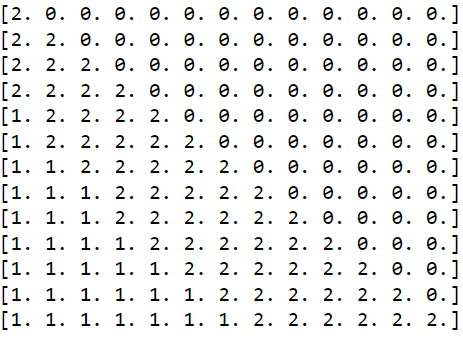
\includegraphics[width=0.7\textwidth]{ArrayBild.PNG}
 \caption{$S_0 = 100, K = 100, r = 0,04, sigma = 0,25 , T = 1, N = 12$}
\end{center}
\end{figure}

 Die Punkte, in denen eine 0 ausgegeben wird, entsprechen keinen wirklichen Knoten des Baumes. Dies sind Punkte, in denen $j > i$ ist. Diese Punkte sind nach Definition ausgeschlossen.

\newpage
Die eins, die pro Periode am weitesten rechts steht, entspricht dem Knoten $(i,B(i))$. Die Folge dieser Knoten bildet also die optimale Ausübungsumgebung 
$ \mathcal{B} = \{ (i,(B(i)) : i \in \mathcal{I} \}$.
\\
In dieser Grafik lässt sich auch gut erkennen, dass es ab der ersten Periode, in der es einen Knoten $(i,B(i))$, in jeder weiteren Periode auch so einen Knoten gibt und, dass es nie 2 Abwärtsbewegungen nacheinander gibt.

\begin{figure}[h]
\begin{center}
 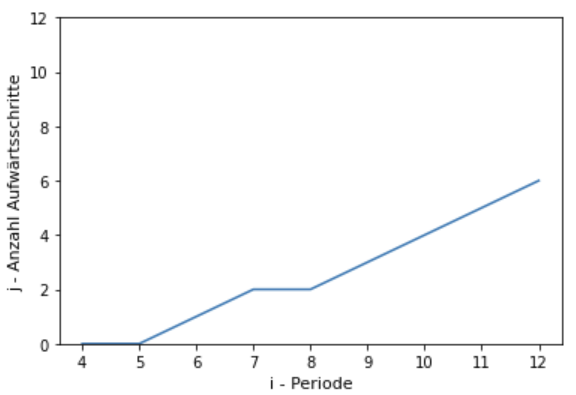
\includegraphics[width=0.7\textwidth]{ArrayBild2.PNG}
 \caption{Optimal Exercise Boundary}
\end{center}
\end{figure}

\newpage
Hier sehen wir noch einmal alle Punkte $(i,B(i))$ des Optimal Exercise Boundary in einer Gerade abgetragen. Der Bereich über der Geraden ist die Hold Region und der Bereich darunter, die Stopping Region.
\\\\
Diese Methode, die Preise der Put Option zu berechnen ist nicht sehr effizient, weil für jeden Knoten (mit Ausnahme von Periode N) Erwartungswert und Auszahlungsprofil miteinander verglichen werden müssen.
\\
Wenn zuerst die optimale Ausübungsumgebung bestimmt wird, können alle Knoten darunter mit $(K - S \cdot u^j \cdot d^{i-j})^+$ und alle Knoten darüber mit dem Erwartungswert ${E}_P(i,j)$ bestimmt werden.
\\\\
Deswegen soll im Folgenden das "Modified Binomial Model" (Kim \& Byun, 1994) vorgestellt werden.


\section{\centering{Modified Binomial Model}}
\subsection{Optimal Exercise Boundary bestimmen}
Zuerst muss der optimale Ausübungsknoten in Periode n, also $(N,B(N))$ bestimmt werden. Es ist klar, dass der Strikepreis $K$ die letzte Periode in die Stopping - und Hold Region unterteilt.
\\
Wir bestimmen also die kleinste Zahl\footnote[3]{Kim and Byum 1994, S.142}  $a$, für das der Preis der Aktie in Periode N größer als der Strikepreis K ist:
\\
\begin{center}
    $S_0\cdot u^a \cdot d^{N-a} > K$
\end{center}

\begin{center}
    $S_0 \cdot u^a \cdot \frac{d^N}{d^a} > K$
\end{center}

\begin{center}
    $\left(\frac{u}{d}\right)^a > \frac{K}{S_0 \cdot d^N}$
\end{center}

\begin{center}
    $a > \frac{ln(\frac{K}{S_0 \cdot d^N})}{ln(\frac{u}{d})}$
\end{center}


Daraus folgt, dass die Knoten $(N,j)$ mit $j < a$ in $S$ liegen und mit 
\\ $(K - S \cdot u^j \cdot d^{N-j})^+$ berechnet werden. Alle Knoten $(N,j)$ mit $j \geq a$ liegen in $H$ und haben den Wert 0, weil $S>K$.
\\
Der optimale Ausübungsknoten in Periode N ist also $(N,B(N)) = (N,a-1)$.
\\
Nun muss der optimale Ausübungsknoten $(N-1,B(N-1))$ bestimmt werden.
\\
Da die optimale Ausübungsumgebung stetig ist, muss $B(N-1) = a-1$ oder $B(N-1) = a-2$ erfüllt sein.
\\
Wir betrachten $P(N-1,a-1)$.
\\
Der Preis in diesem Knoten entspricht:
\begin{center}
    $max[\frac{p}{R} \cdot P(N,a) + \frac{1-p}{R} \cdot P(N,a-1), K - S_0\cdot u^{a-1} \cdot d^{N-a}]$ 
\end{center}

\begin{center}
    $max[\frac{1-p}{R} \cdot (K-S_0 \cdot u^{a-1} \cdot d^{N-a+1}, K - S_0\cdot u^{a-1} \cdot d^{N-a}]$ 
\end{center}

wobei\\ $\frac{p}{R} \cdot P(N,a)$ entfällt, da $P(N,a) = 0$ und  $P(N,a-1) = (K-S_0^{a-1} \cdot d^{N-a+1})$

\newpage

$B(N-1)$ ist also $a-1$ falls:
\begin{center}
    $K - S_0\cdot u^{a-1} \cdot d^{N-a} \geq \frac{1-p}{R} \cdot (K-S_0 \cdot u^{a-1} \cdot d^{N-a+1}) $ 
\end{center}

\begin{center}
    $K \geq \left(\frac{p}{R-1+p}\right) \cdot S_0\cdot u^{a} \cdot d^{N-a}$ 
\end{center}

Daraus ergibt sich:
\\\\
$B(N-1)$ = \begin{cases}
    $a - 1$     & \text{ falls } $\left(\frac{p}{R-1+p}\right) \cdot S_0\cdot u^{a} \cdot d^{N-a} \leq K < S_0\cdot u^{a} \cdot d^{N-a}$\\
    $a - 2$  & \text{ falls } $S_0\cdot u^{a-1} \cdot d^{N-a+1} \leq K < \left(\frac{p}{R-1+p}\right) \cdot S_0\cdot u^{a} \cdot d^{N-a}$ 
\end{cases}
\\\\\\
Es folgt ebenfalls, dass es einen kritischen Aktienpreis $S^*_{N-1}$ gibt, der sich mit den verwendeten Variablen definieren lässt. $S^*_{N-1}$ ist der Preis, für den gilt, dass wenn $S_{N-1} < S^*_{N-1}$, die Put Option sofot ausgeübt werden sollte.
\\\\
$S^*_{N-1}$ ist definiert als:
\begin{center}
    $S^*_{N-1} = [1 - \frac{(1-p) \cdot (1-d)}{p \cdot u} ] \cdot K$ 
\end{center}

Sodass:
\\\\
$B(N-1)$ = \begin{cases}
    $a - 1$     & \text{ falls } $S^*_{N-1} \geq S_0\cdot u^{a-1} \cdot d^{N-a}$\\ 
    $a - 2$     & \text{ falls } $S^*_{N-1} < S_0\cdot u^{a-1} \cdot d^{N-a}$
\end{cases}
\\\\\\
Mit dem gleichen Vorgehen lässt sich auch $B(N-2)$ bestimmen.
\\\\
Für $S^*_{N-2}$ ergibt sich:
\begin{center}
    $S^*_{N-2} = [1 - \frac{R \cdot (1-p) \cdot (1-d)}{(p \cdot u)^2} ] \cdot K$
\end{center}

Sodass:
\\\\
$B(N-2)$ = \begin{cases}
    $a - 2$     & \text{ falls } $S^*_{N-2} \geq S_0\cdot u^{a-2} \cdot d^{N-a}$\\ 
    $a - 3$     & \text{ falls } $S^*_{N-2} < S_0\cdot u^{a-2} \cdot d^{N-a}$
\end{cases}

\newpage

Sei nun $N_1$ die erste Periode, in der $B(N_1) = B(N_1 + 1)$ gilt, wenn man rückwärts durch den Baum geht.
\\
Sei außerdem $i_1 = N - N_1$. Wenn wir das Beispiel aus Abbildung 4 - und 5 betrachten, ist $N_1 = 7$, da $B(7) = B(8) = 2$.
\\
Es ergibt sich also mit $N = 12$ und $N_1 =7 $, $i_1 = 12 - 7 = 5$
\\\\
Daraus folgt, dass
\\
$B(N) = a - 1$, $B(N-1) = a - 2$, $B(N-2) = a - 3$, $B(N-3) = a - 4$ , $B(N-4) = a - 5$, $B(N-5) = a - 5$
\\\\

$i_1$ ist die kleinste positive Zahl, für die
\begin{center}
    $K \cdot [1-\left(\frac{1-p}{R}\right) \cdot \left(\frac{1-\left(\frac{p}{R}\right)^{i_1}}{1-\frac{p}{R}}\right)] \geq S_0 \cdot u^a \cdot d^{N-a} \cdot \left(\frac{p}{R}\right)^{i_1}$
\end{center}
gilt.
\\\\
Daraus folgt für $i_1$:

\begin{center}
    $i_1 \geq \frac{ln \left(\frac{K^'}{S_0 \cdot u^a \cdot d^{N-a} - K + K^'}\right)}{ln \left(\frac{p}{R}\right)}$
\end{center}

wobei $K' = K \cdot \left(\frac{R-1}{R-p}\right)$ entspricht.
\\\\
Die Punkte $B(i)$ lassen sich von $N_1$ bis $N$ wie folgt berechnen, sobald $i_1$ gefunden ist:
\\\\
$B(Ni)$ = \begin{cases}
    $B(N) - (N-1)$     & \text{ falls } $N_1 < i \leq N $\\ 
    $a - (N - 1)$     & \text{ falls } $i = N_1$
\end{cases}

\newpage

Nach diesem Schema lässt sich auch $N_2$ bestimmen. Wenn $N_2$ der zweite Zeitpunkt in der Rückwärtsbetrachtung ist, zu dem $B(N_2) = B(N_2 + 1)$, dann ist $i_2 = N_1 - N_2$.
\\\\
Für $i_2$ gilt:
\begin{center}
       $ i_2 \geq \frac{ln \left(\frac{K^'}{S_0 \cdot u^a \cdot d^{N-a} - K + K^'}\right)}{ln \left(\frac{p}{R}\right)}$.
\end{center}
 \\\\


Jetzt wird eine allgemeine Formel definiert, um den optimalen Knoten im Zeitpunkt $N_k$ zu finden, wobei $k = 0,1,2...$ das k`te mal in der Rückwärtsbetrachung ist, zu dem $B(N_k) = B(N_k + 1)$ ist. \\\\
Sei $N_0 = N, a_0 = a$, dann ist $i_k = N_{k-1}-N_{k}$ und $a_k = a_{k-1} - i_k +1 $, wobei $k= 0,1,2,...$. \\
$i_{k+1}$ wird definiert als: \\
\begin{center}
  $i_{k+1} \geq \frac{ln \left(\frac{K^'}{d(N_k,a_k) + K^'}\right)}{ln \left(\frac{p}{R}\right)} $  
\end{center}
   

\\[0,3 cm]
wobei $d(N_k,a_k)= P(N_k,a_k) - (K - S \cdot u^a_k \cdot d^{N_k-a_k})$ den Zeitwert von der Amerikanischen Put-Option im Zeitpunkt $(N_k,a_k)$ bezeichnet.
Danach können $N_{k+1}$ und $a_{k+1}$ berechnet werden als:
$N_{k+1} = N_k - i_{k+1}$ und $a_{k+1} = a_k - i_{k+1} +1$. \\\\
Sei $ \mathcal{B}(N_k) = a_k -1$ der Ausübungszustand für jedes $N_k, k= 0,1,2,...$, dann ist $(N_k, \mathcal{B}(N_k))$ die Menge der \textbf{Optimal Exercise Boundary}. 

\subsection{Amerikanischen Put Preis bestimmen}
Mit der Hilfe von der \textbf{Optimal Exercise Boundary} wird \\der Amerikanischen Put Preis in der Endperiode N definiert als: \\

\begin{center}
    \textbf{P(N,j)} = 
\begin{cases}
    $0     & \text{ für } (N,j) \in \mathcal{H}$\\
    $K - S \cdot u^{a-1} \cdot d^{N-a+1} & \text{ für } (N,a-1) \in \mathcal{B} $
\end{cases}   
\end{center}
\newpage
Für andere Zeitpunk $i<N$ gilt: \\

\begin{center}
    \textbf{P(i,j)} = 
\begin{cases}
    $ \mathbb{E}_P(i,j)$ & \text{ für } $(i,j) \in \mathcal{H}$\\
    $K - S \cdot u^{j} \cdot d^{i-j}$ & \text{ für } $(i,j) \in \mathcal{B}. $
\end{cases} 
\end{center}
Das heißt:\\

\begin{center}
    \textbf{P(i,j)} = 
\begin{cases}
    \frac{p}{R} \cdot P(i+1,j+1) \cdot \frac{1-p}{R} \cdot P(i+1,j)& \text{ für } $(i,j) \in \mathcal{H}$\\
    K - S \cdot u^{j} \cdot d^{i-j} & \text{ für } $(i,j) \in \mathcal{B}. $
\end{cases} 
\end{center}
Mit dieser Formel\footnote[4]{Kim and Byun 1994, S.150} versteht man, dass die Amerikanische Put Option in einem Knoten (i,j) den Wert des Erwartungswertes $ \mathbb{E}_P(i,j)$ annimmt, wenn der Knoten in der Hold Region liegt. Wenn der Knoten (i,j) ein Boundary Knoten ist, dann wird der Preis der Option mit dem Auzahlungsprofil berechnet. 

\newpage 

\subsection{Modellierung in Python}

Als erstes wird eine Funktion Put() definiert, die den Preis der Option in einem bestimmten Knoten (nk,ak) berechnet und ihn zurückgibt.
\\\\
Danach erstellen wir eine Funktion timevalue(), die den Zeitwert der Put-Option in einem bestimmten Knoten berechnet. Der Zeitwert ergibt sich aus der Differenz zwischen dem Wert der Option und dem Auszahlungsprofil. Diesen werden wir später brauchen um die verschiedenen $i_k$ zu berechnen.
\\\\
Als drittes haben wir die BoundaryKnoten() Funktion erstellt. Hier werden die verschiedenen Werte für $i_k, n_k$ und $a_k $ berechnet. Das ganze wird mit einer For-Schleife gemacht. In der Schleife wird jedes $i_k$ berechnet. Falls das Ergebnis von $i_k \leq N$  ist, wird damit das nächste $n_k$ und $a_k$ bestimmt. Die Schleife wird unterbrochen, sobald $a_{k+1} \leq 0$ ist, weil dann der letzte Boundary Knoten erreicht wurde.
\\\\
Darauf folgend wird die Funktion FillTheSquare() definiert. Diese Funktion erstellt einen Array EmptySquare, in dem auf Basis der $i_k, n_k$ und $a_k$ die Boundary Knoten eingetragen werden. In der folgenden Grafik sehen wir den Output der Funktion.
\\\\
\begin{figure}[h]
\begin{center}
 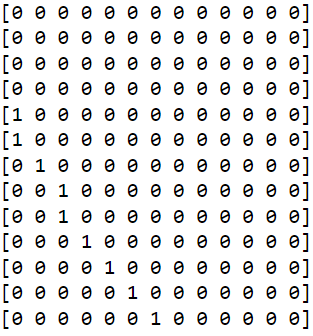
\includegraphics[width=0.33\textwidth]{FillTheSquare.PNG}
 \caption{FillTheSquare() Output}
\end{center}
\end{figure}

Die letzte Funktion ist die PutBoundary Funktion. Mit dieser Funktionen kann nun der Put-Preis in einem bestimmten Knoten auf Basis der Optimal Exercise Boundary berechnet werden. 

\part{Fazit}

In diesem Projekt ging es um die Optimal Exercise Boundary von amerikanischen Put Optionen. Die Optimal Exercise Boundary definiert die Grenze zwischen zwei Regionen, der Hold - und Stopping Region. Anhand dieser Grenze kann der Investor entscheiden, ob es von Vorteil ist, die Option auszuüben oder sie weiter zu halten.
\\\\
Um den Preis von amerikanischen Put Optionen in einem Binomial Modell zu bestimmen, muss immer dar Erwartungswert $E_p$ bestimmt und mit dem Auszahlungsprofil $K-S$ verglichen werden. Wenn aber zuerst die Optimal Exercise Boundary bestimmt wird, können die Put Preise schneller berechnet werden, weil alle Punkte darüber mit $E_p$ und alle Punkte darauf bzw. darunter mit dem Auszahlungsprofil berechnet werden.
\\\\
\part{Aufgabenverteilung}
Das Protokoll und auch der Code wurde gleichermaßen von Minh Anh Le und Leander Piepenbring verfasst.
\newpage
\part * { Literaturverzeichnis }
\addcontentsline{toc}{part}{Literaturverzeichnis}

\big[Kim/Byun 1994\big] \bfseries\itshape\underline{}{Optimal Exercise Boundary in a Binomial Option Pricing Model},\mdseries \\ {https://www.researchgate.net/publication/249961195\_Optimal\_Exercise\_Boundary\\\_in\_a\_Binomial\_Option\_Pricing\_Model, letzter Stand: 28.03.2022}. \\

\big[Prof.Dr. Christina Erlwein-Sayer 2021\big] \bfseries\itshape\underline{}{Vorlesungskript Thema Binomial Modell und Amerikanische Optionen},\mdseries \\
{letzter Stand:28.03.2022}. \\

\big[Basso 2001\big] \bfseries\itshape\underline{}{Discrete and continuous time approximations of the optimal exercise boundary of American options},\mdseries\\ {https://www.researchgate.net/publication/254633761\_Discrete\_and\_continuous\_time\\\_approximations\_of\_the\_optimal\_exercise\_boundary\_of\_American\_options,\\ letzter Stand:28.03.2022}. \\ 

\big[Kpmoony 2021\big] \bfseries\itshape\underline{}{Numerical Methods Binomial Modell},\mdseries\\
{https://github.com/kpmooney/numerical\_methods\_youtube/blob/master\\\/binomial\_model/Binomial\%20Model.ipynb, letzter Stand:28.03.2022}. \\

\big[Sheikh Pancham 2021\big] \bfseries\itshape\underline{}{Python Implementation Binomial},\mdseries\\
{https://www.linkedin.com/pulse/python-implementation-binomial-stock-option-pricing-sheikh-pancham, letzter Stand:28.03.2022}. \\

\big[James Ma Weiming 2015\big] \bfseries\itshape\underline{}{Mastering Python for Finance},\mdseries \\
{https://www.palmislandtraders.com/econ136/mpff.pdf, letzter Stand:28.03.2022}.\\

\end{text}
\end{document}
